\begin{figure*}

\begin{minipage}{0.33\linewidth}
  \centering
  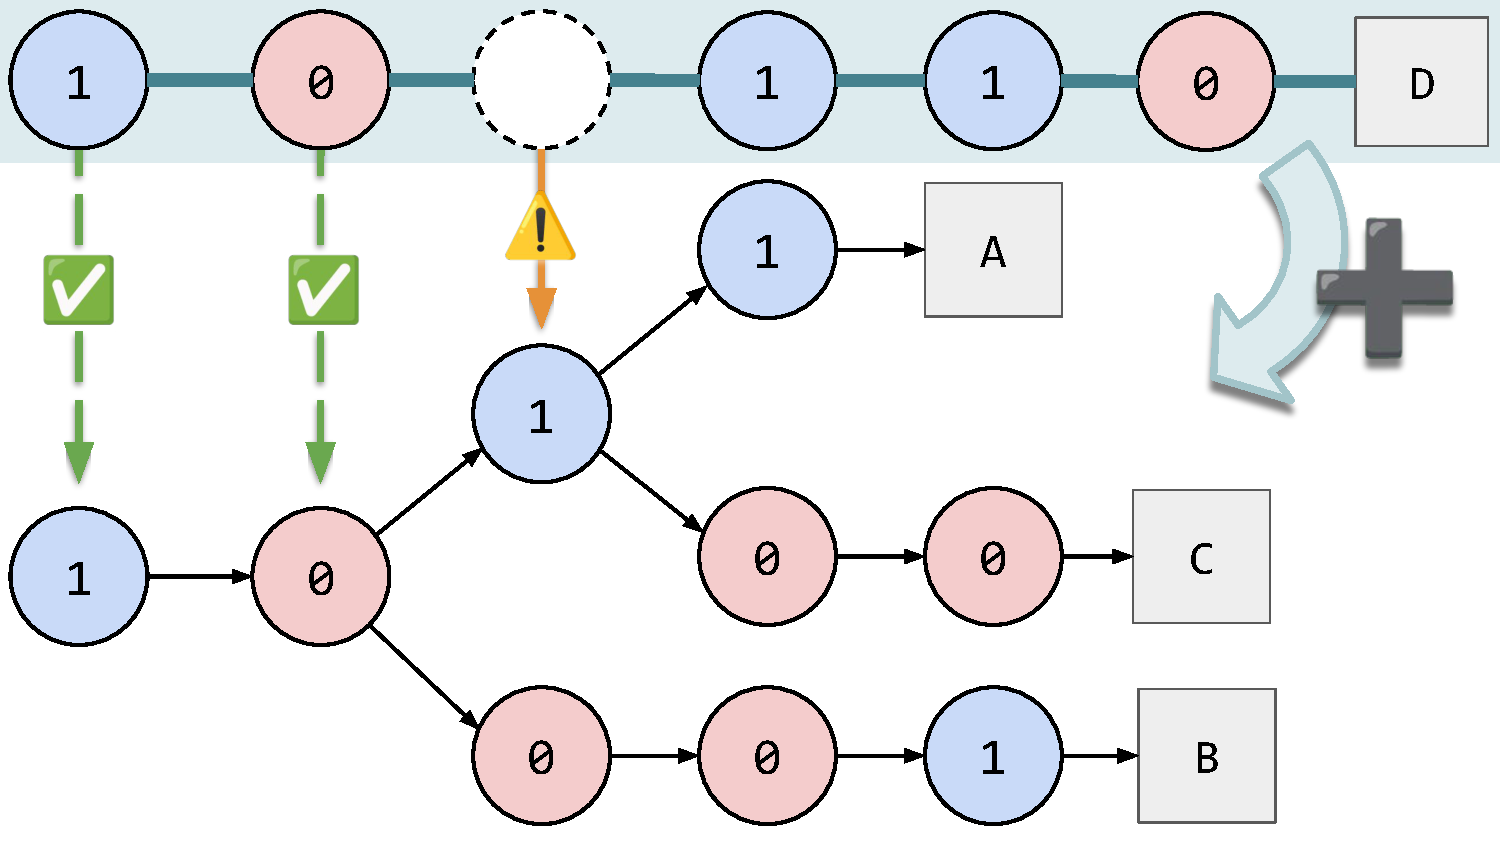
\includegraphics[width=\linewidth]{img/shortcut-algo-diagram-1}
  \subcaption{Preparing to add organism D}
\end{minipage}
\begin{minipage}{0.33\linewidth}
  \centering
  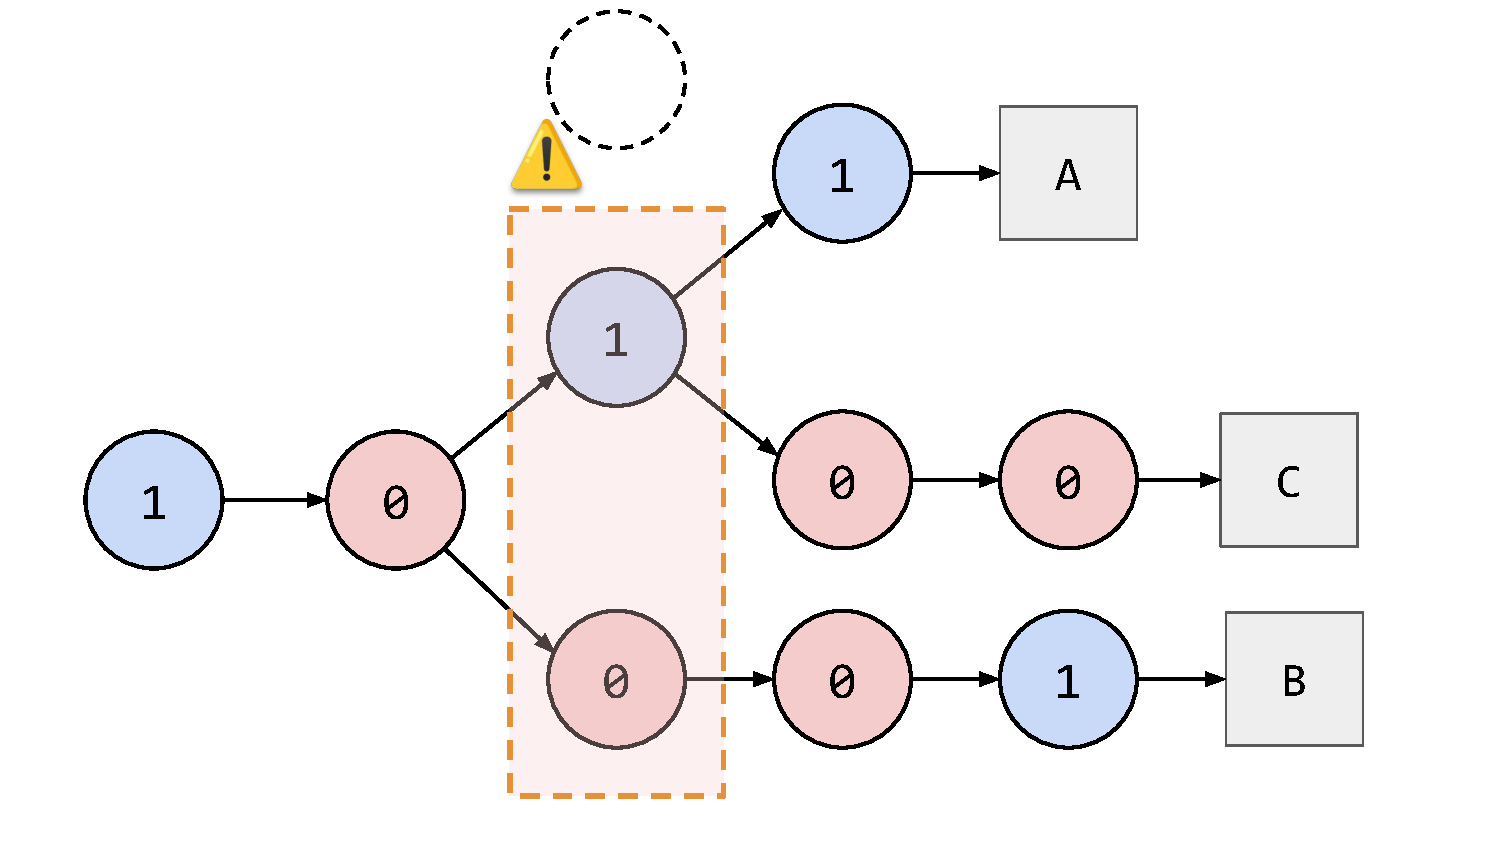
\includegraphics[width=\linewidth]{img/shortcut-algo-diagram-2}
  \subcaption{Recognizing outdated information}
\end{minipage}
\begin{minipage}{0.33\linewidth}
  \centering
  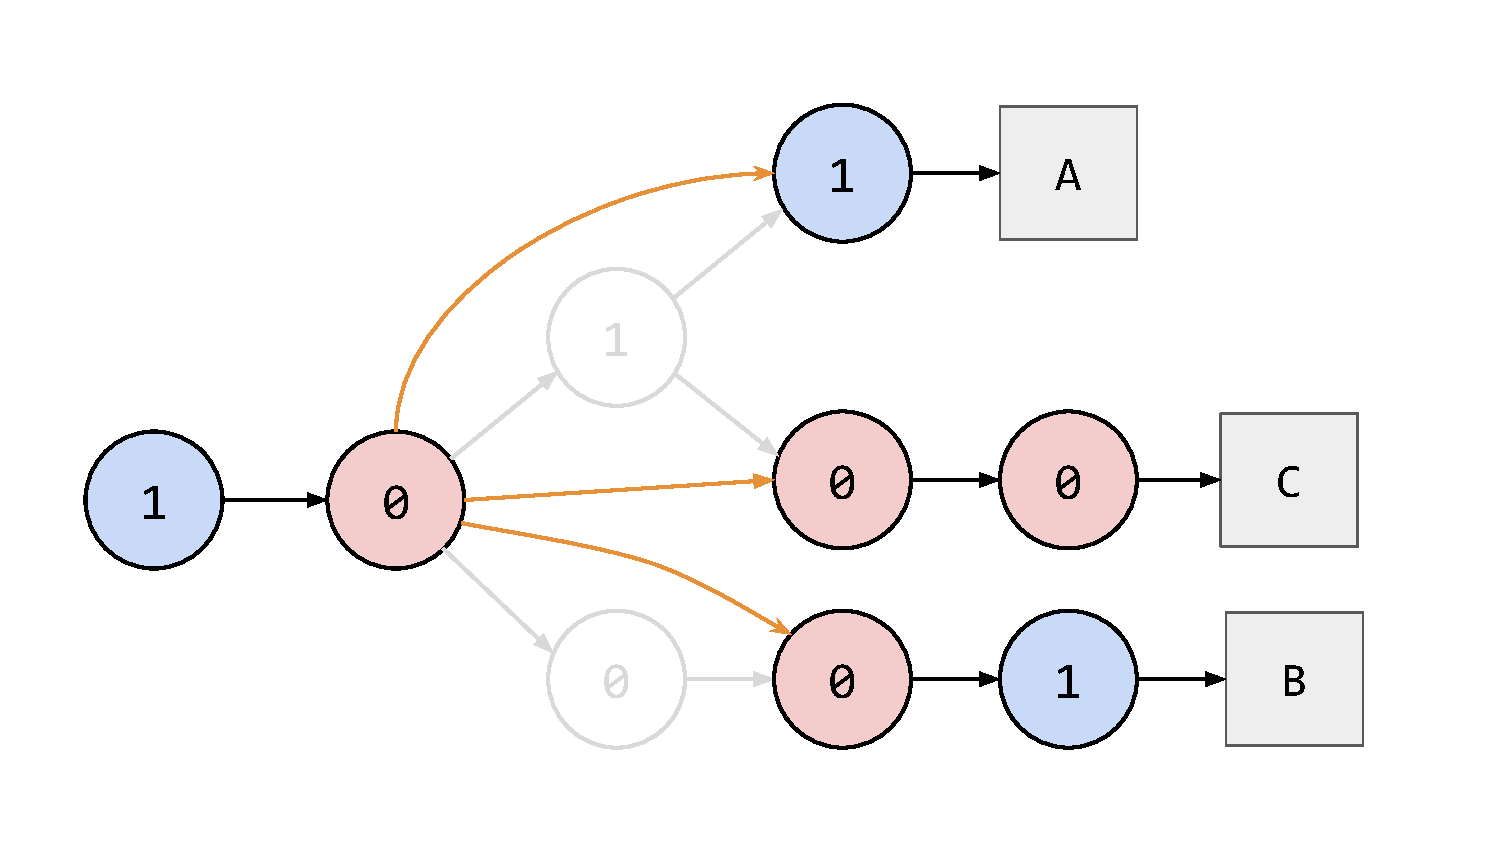
\includegraphics[width=\linewidth]{img/shortcut-algo-diagram-3}
  \subcaption{Creation of shortcuts}
\end{minipage}

\begin{minipage}{0.33\linewidth}
  \centering
  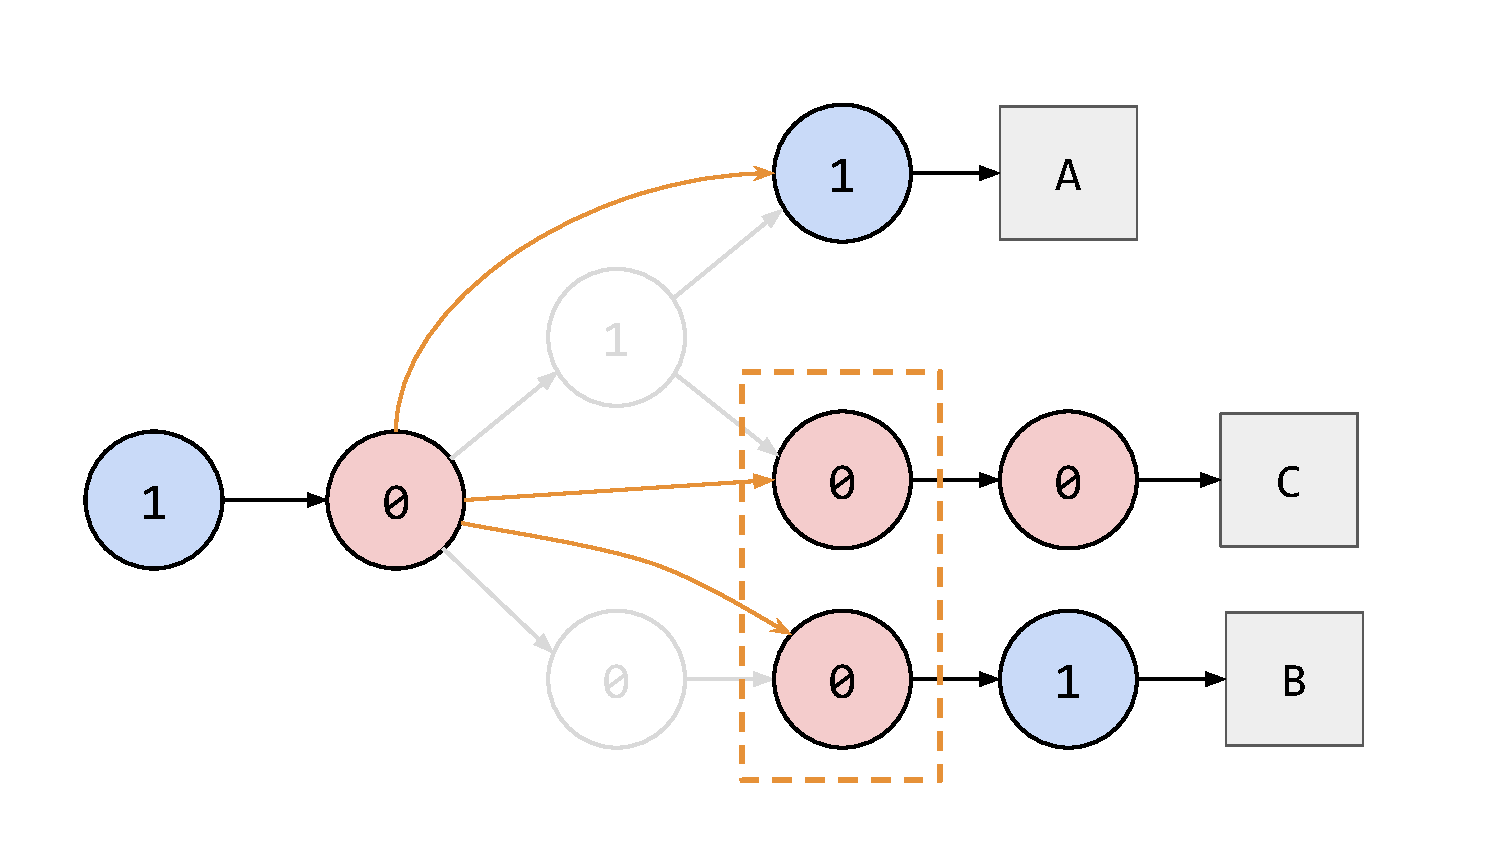
\includegraphics[width=\linewidth]{img/shortcut-algo-diagram-4}
  \subcaption{Recognizing duplicates by shortcut}
\end{minipage}
\begin{minipage}{0.33\linewidth}
  \centering
  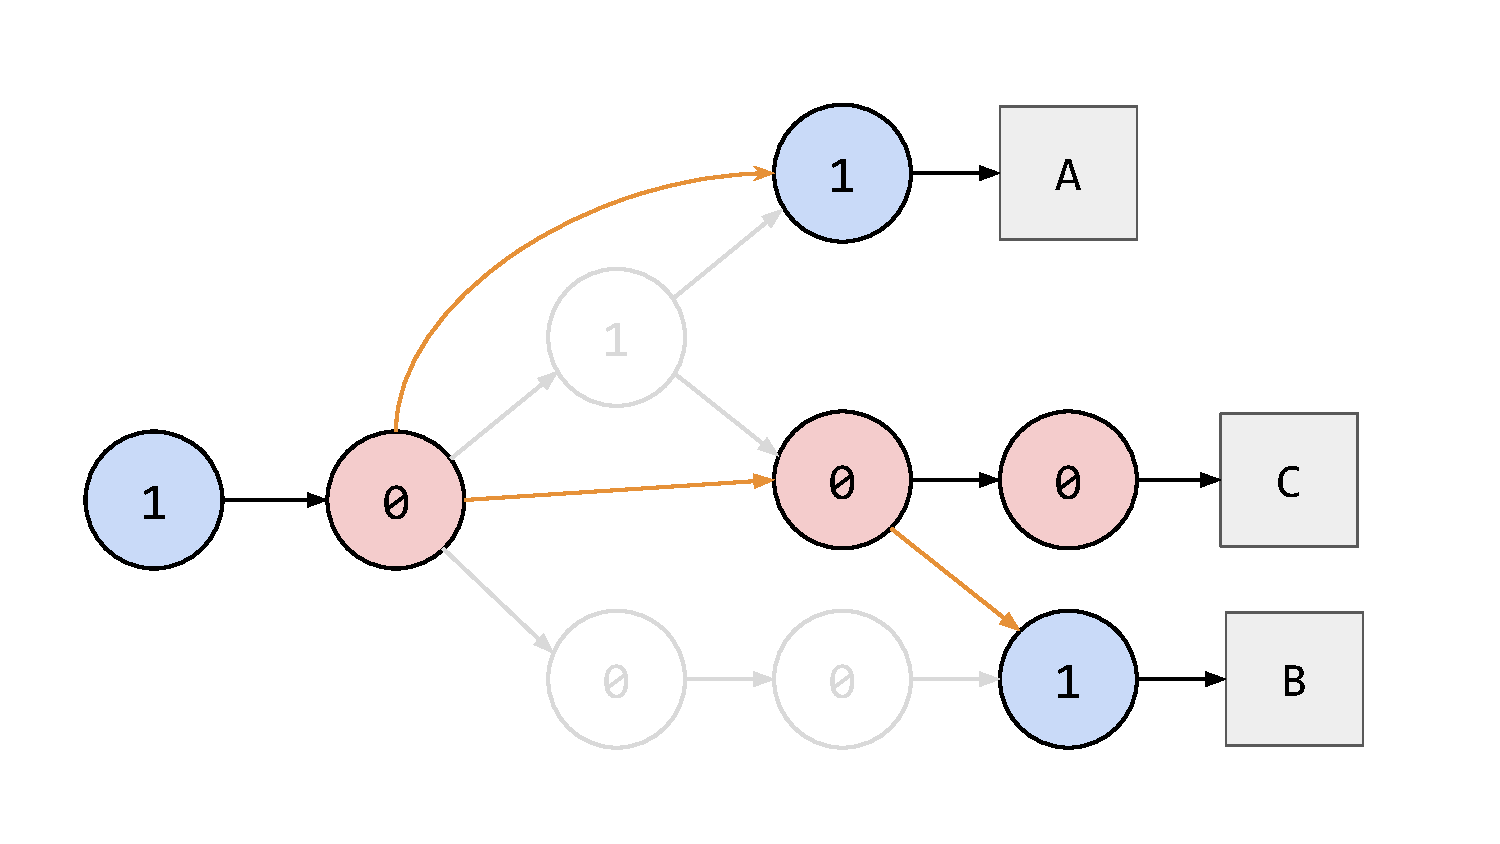
\includegraphics[width=\linewidth]{img/shortcut-algo-diagram-5}
  \subcaption{Collapsing indistinguishable nodes}
\end{minipage}
\begin{minipage}{0.33\linewidth}
  \centering
  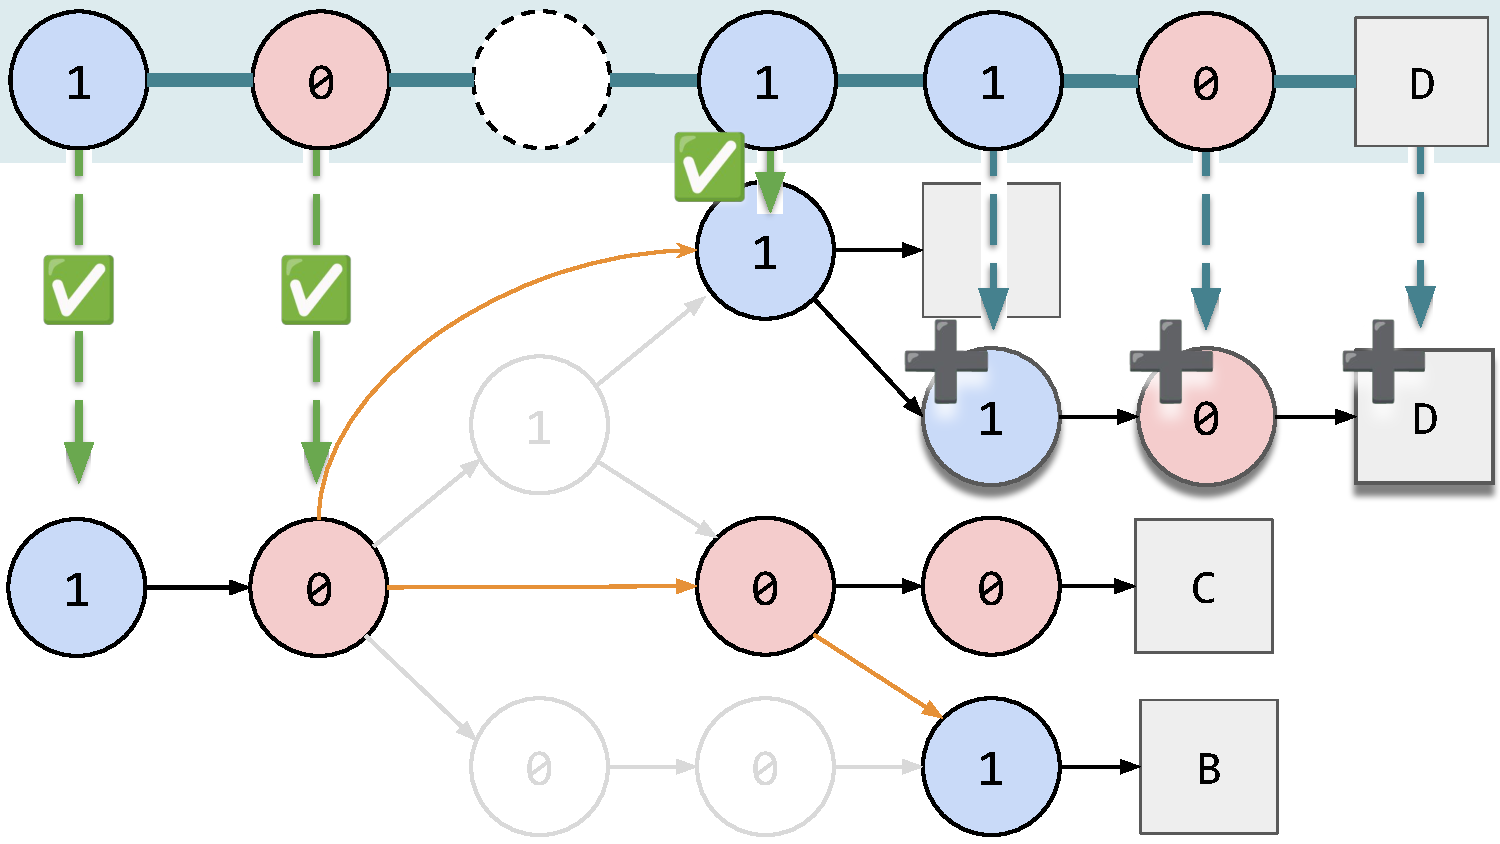
\includegraphics[width=\linewidth]{img/shortcut-algo-diagram-6}
  \subcaption{Adding organism D}
\end{minipage}
\caption{\textbf{The shortcut algorithm dealing with missing information.} In steps (b) and (c), the missing information is consolidated and shortcuts are built around it. In steps (d) and (e), duplicates are resolved by merging them together and building more shortcuts.}
\label{fig:algo-diagram}

\end{figure*}